\documentclass[9pt]{report}

\usepackage{talks}

\begin{document}

\sf%
\mbox{ }
\\[12pt]
\spc{\LARGE\bfseries \color{MidnightBlue}{From 0 to 100K in 10 years:}}
\\[4pt]
\spc{\Large\bfseries \color{MidnightBlue}{nurturing open-source community}}
\\[36pt]
\noindent 
\spc{\large\bfseries \color{MidnightBlue}{Bob Carpenter}}
\\[2pt]
\spc{\small Center for Computational Mathematics}
\\[2pt]
\spc{\small Flatiron Institute}
\vfill 
\noindent 
\spc{\footnotesize June 2024: U. Ljubljana}
\hfill 
{\footnotesize \url{https://mc-stan.org}}
\hfill 

\includegraphics[width=0.3in]{img/new-logo.png}

\sld{Taking uncertainty seriously}
\begin{itemize}
\item \myemph{Uncertainty} permeates science and decision making:
  \begin{subitemize}
  \item \myemph{sampling} uncertainty
    \begin{subitemize} \item data is finite \end{subitemize}
  \item \myemph{measurement} uncertainty
    \begin{subitemize} \item measurements are noisy, biased, and incomplete \end{subitemize}
  \item \myemph{modeling} uncertainty
    \begin{subitemize} \item our models are imperfect reflections of
      reality \end{subitemize}
  \end{subitemize}
  \vfill
\item The alternative to \myemph{good statistics} is
  not no statistics,
  but \myemph{bad statistics}. \hfill \small{(Bill James)}
\end{itemize}

\sld{Probability \& Statistics}
\begin{itemize}
\item Probability theory uses math to \myemph{quantify uncertainty}.
\item \myemph{Bayesian statistics} applies probability theory to
  \begin{subitemize}
  \item data {analysis}
  \item inference (estimation and prediction)
  \item model {evaluation} and comparison
  \item {decision} theory (given preferences)
  \end{subitemize}
\item The \myemph{computational bottlenecks} for Bayes are
  \begin{subitemize}
  \item model expression
  \item posterior inference
  \end{subitemize}
\end{itemize}


% \sld{Probability is \textit{\bfseries not} $\ldots$}
% {\linespread{1.3}
% \small\linespread{1.35}
% \begin{quote}\linespread{1.5}An intellect which at a certain
%   moment would know all forces that set nature in motion, and all
%   positions of all items of which nature is composed, if this
%   intellect were also vast enough to submit these data to analysis, it
%   would embrace in a single formula the movements of the greatest
%   bodies of the universe and those of the tiniest atom; \myemph{for such an
%   intellect nothing would be uncertain} and the future just like the
%   past would be present before its eyes.
%   \vfill\linespread{1.25}
%   -- \footnotesize \myemph{Pierre-Simon Laplace}. 1814.  \textit{A
%   Philosophical Essay on Probabilities}.  Translated by
%   F.~W.~Truscott and F.~L.~Emory, 1951.  
% \end{quote}
% }


\sld{Bayesian probability is epistemic}
{\linespread{1.3}
  \small
  \begin{quote}
    \myemph{Every event is
      in itself certain, not probable}; if we knew all, we should either know
    positively that it will happen, or positively that it will not. But
    its \myemph{probability} to us means the \myemph{degree of expectation} of its
    occurrence, which we are \myemph{warranted in entertaining} by our present
    \myemph{evidence}.
    \vfill\linespread{1.25}
    -- \footnotesize \myemph{John Stuart Mill}.  1882.  \textit{A System
      of Logic: Ratiocinative and Inductive}. Eighth edition.  III:18.
  \end{quote}
}



\sld{Bayesian modeling}
\begin{itemize}
\item Define a \myemph{generative model} for data $y$ and parameters
  $\theta$ as a probability density $p(y \mid \theta)$
  \begin{subitemize}
  \item e.g., compose a forward scientific model and a measurement model
  \end{subitemize}
\item Define our present evidence as a \myemph{prior} density
  $p(\theta)$, e.g., 
  \begin{subitemize}
  \item realistic ranges of cancer prevalence,
  \item possible masses of exoplanets,
  \item livable metabolic rates for humans,
  \item concentration of particulates in breathable air,
  \item realistic major league batting averages,
  \item and so on
  \end{subitemize}
\end{itemize}

\sld{Bayesian inference}
\begin{itemize}
\item Observe actual \myemph{data} $y$
\item Calculate expectations over the \myemph{posterior}
  \[
    p(\theta \mid y) \propto p(y \mid \theta) \cdot p(\theta)
  \]
  \begin{subitemize}
  \item parameter estimation $\widehat{\theta} = \mathbb{E}[\theta \mid y]$
  \item forecasting events $\textrm{Pr}[E \mid y] = \mathbb{E}[\textrm{I}(\theta \in E) \mid y]$
  \item predictions for new data: $p(\tilde{y} \mid y) =
    \mathbb{E}[p(\tilde{y} \mid \theta) \mid y]$
  \end{subitemize}
\item Estimate with \myemph{Markov chain Monte Carlo (MCMC)} (or approximations)
\end{itemize}


\sld{What is Stan?}
% 
\begin{itemize}
\item a domain-specific \myemph{probabilistic programming language}
\item Stan \myemph{program} defines a \myemph{differentiable} probability model
  \begin{subitemize}
  \item declares data and (constrained) parameter variables
  \item defines log posterior (or penalized likelihood)
  \item defines predictive quantities
  \end{subitemize}
\item Stan \myemph{inference} fits model \& makes predictions
  \begin{subitemize}
  \item MCMC for full Bayesian inference
  \item variational and Laplace for approximate Bayes
  \end{subitemize}
\item \footnotesize Carpenter, B., Gelman, A., Hoffman, M. D., Lee, D., Goodrich, B., Betancourt, M., Marcus Brubaker, Jiqiang Guo, Peter Li, Riddell, A. (2017). Stan: A probabilistic programming language. {\slshape J.\ Stat.\ Soft.} 76(1).
\end{itemize}

\sld{e.g., Logistic Regression}
% 
\begin{stancode}
  data {
    int<lower=1> K;
    int<lower=0> N;
    matrix[N,K] x;
    int<lower=0,upper=1> y[N];
  }
  parameters {
    vector[K] beta;
  }
  model {
    beta ~ cauchy(0, 2.5);          // prior
    y ~ bernoulli_logit(x * beta);  // likelihood
  }
\end{stancode}

\sld{\large Holographic coherent diffraction imaging}
\begin{itemize}
\item \small Brian Ward (CCM) and I reproduced David Barmherzig's
  paper to illustrate Stan's complex number and FFT capability
\item \footnotesize GitHub: \myemph{\texttt{bob-carpenter/CDI}}
\end{itemize}
\begin{center}
  
\includegraphics[width=0.51\textwidth]{img/barmherzig-cite.png}
\end{center}


\sld{Holo CDI (1)}
\begin{itemize}
\item \small Step 1: direct \myemph{coherent radiation} source (e.g., X-ray) at
  biomolecule and target \& uniformly redundant array (URA)
  \myemph{reference}, with \myemph{beam stop}; (data
  \myemph{simulated}, but works with real)
\end{itemize}
\vspace*{-8pt}
\begin{center}
  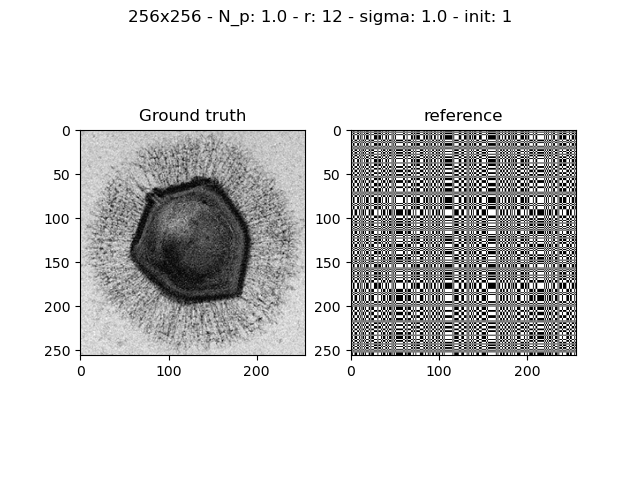
\includegraphics[width=0.6\textwidth]{img/fft/truth-ref.png}
\end{center}


\sld{Holo CDI (2)}
\vspace*{-2pt}
\begin{itemize}
\item \small Step 2: observe diffracted \myemph{photon counts} $\tilde{Y}_{i,j}$
  \begin{subitemize}
  \item beamstop visible in middle (low frequencies)
    % \item  plot is $\log (1 + Y_{i,j})$; obs. low
  \end{subitemize}
\end{itemize}
\vspace*{-8pt}
\begin{center}
  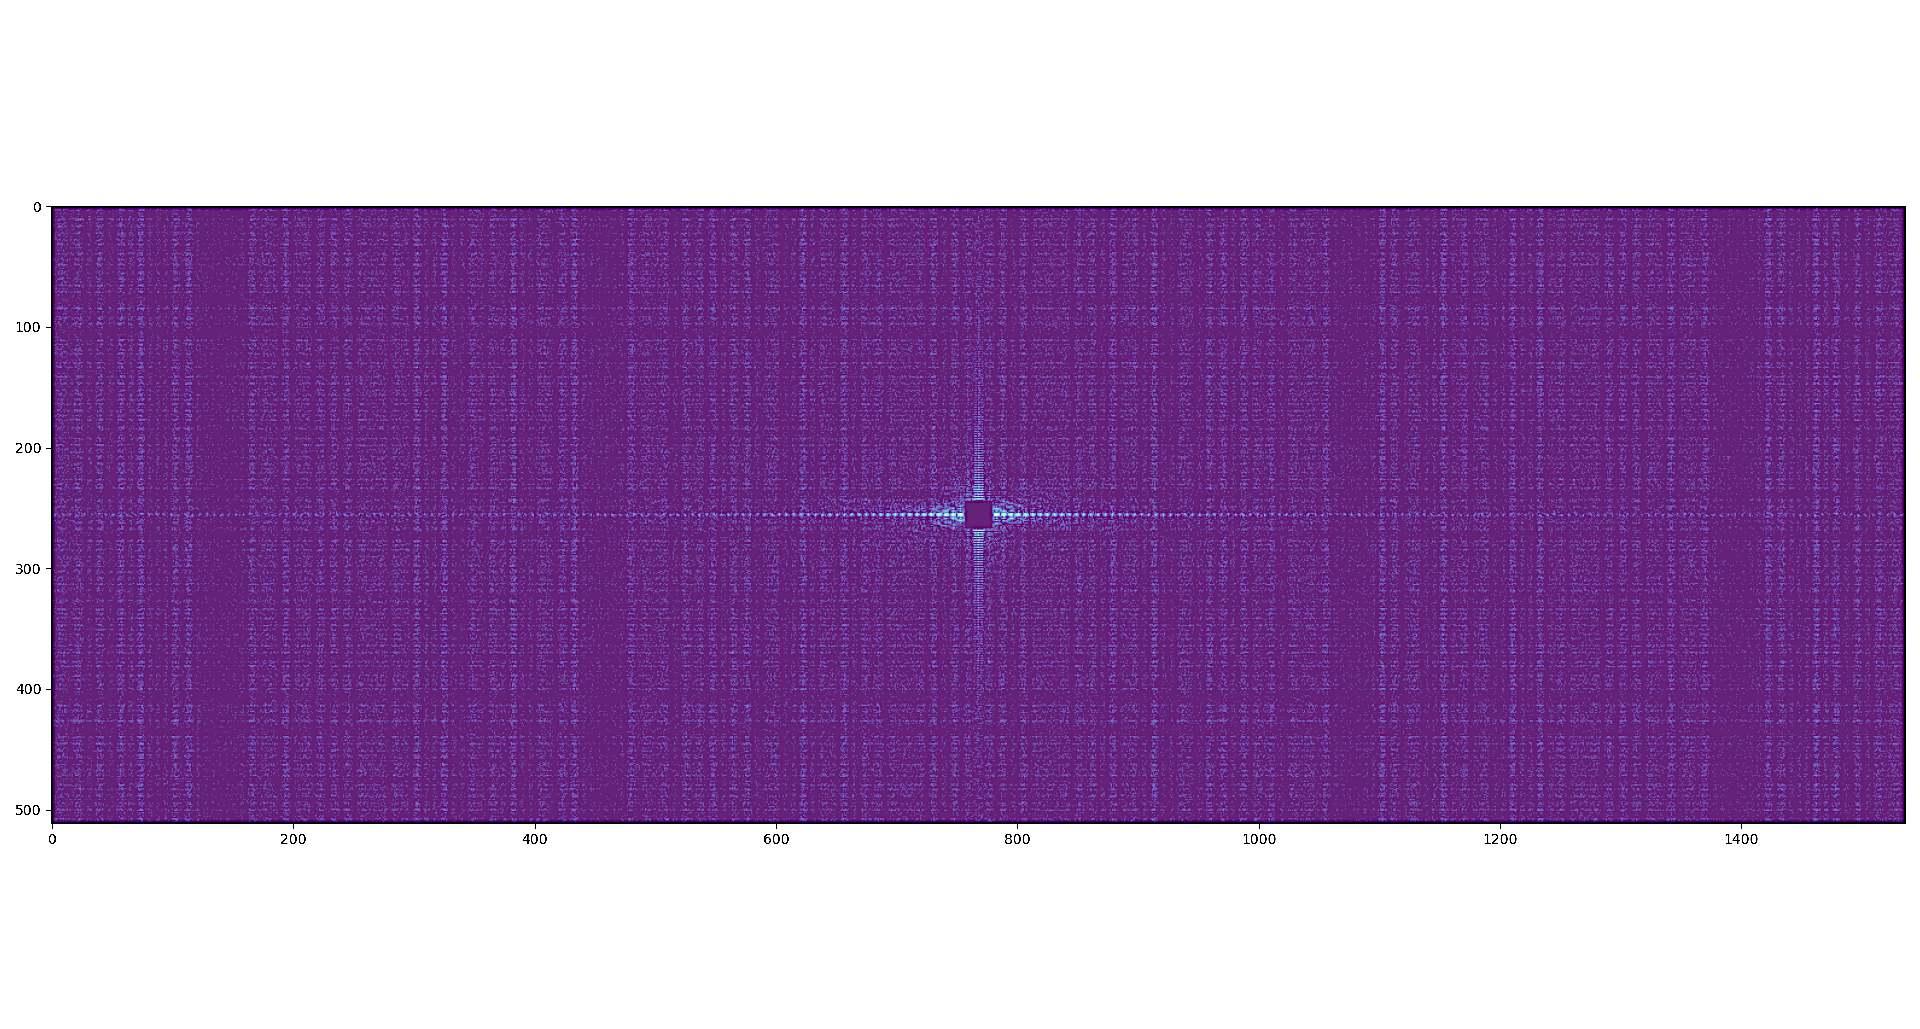
\includegraphics[width=0.9\textwidth]{img/fft/observed.png}
\end{center}

\sld{Holo CDI (3.a)}
\begin{itemize}
\item Step 3.a: code \myemph{data format} in Stan (simplified)
  \footnotesize
\begin{verbatim}
data {
  int<lower=0> N;                      // image dim
  matrix<lower=0, upper=1>[N, N] R;    // registration img
  int<lower=N> M1;                     // padded rows
  int<lower=3 * N> M2;                 // padded cols
  int<lower=1, upper=M1> r;            // beam stop size
  real<lower=0> N_p;                   // avg photons/pixel
  array[M1, M2] int<lower=0> Y_tilde;  // observed photons
}
\end{verbatim}
\end{itemize}
  
\sld{Holo CDI (3.b)}
\begin{itemize}
\item \small Step 3.b: code \myemph{transformed data, parameters, and likelihood}
  \footnotesize
\begin{verbatim}
transformed data {
  matrix[M1, M2] B_stop = pad(M1, M2, r);  // beam stop
}
parameters {
  matrix<lower=0, upper=1>[N, N] X;       // image pixels
}
model {
  matrix[M1, M2] X0R_pad = pad(X, R, M1, M2);
  matrix[M1, M2] E_Y = B_stop .* abs(fft2(X0R_pad)) .^ 2;
  matrix[M1, M2] lambda = N_P / mean(Y) * E_Y;

  Y_tilde ~ poisson(lambda);  // likelihood
  X ~ uniform(0, 1);          // prior
}
\end{verbatim}
\end{itemize}

\sld{Holo CDI (4)}
\begin{itemize}
\item Turn Stan's crank to solve the \myemph{inverse problem}
\item using state-of-the-art \myemph{gradient-based inference}: 
  \begin{subitemize}
  \item maximum likelihood via quasi-Newton optimization (L-BFGS)
  \item full Bayes via Markov chain Monte Carlo sampling (NUTS)
  \item approximate Bayes via black-box variational inference (ADVI)
  \end{subitemize}
\item For the \myemph{$256 \times 256$} pixel reconstructions in David's paper,
  \begin{subitemize}
  \item optimization solves inverse problem in \myemph{2 minutes}
  \item sampling solves inverse problem in \myemph{2 hours}
  \end{subitemize}
\item Full study considers L1 \& L2 regularizing \myemph{spatial
    priors} (penalize diffs in adjacent pixels)
\end{itemize}  

\sld{Holo CDI (5.a)}
\begin{itemize}
\item Recovered images $X^*$ at $256 \times 256$ with
  \\ 1 photon/pixel (left)
  vs.\ 10 photons/pixel (right)
\end{itemize}
\begin{center}
  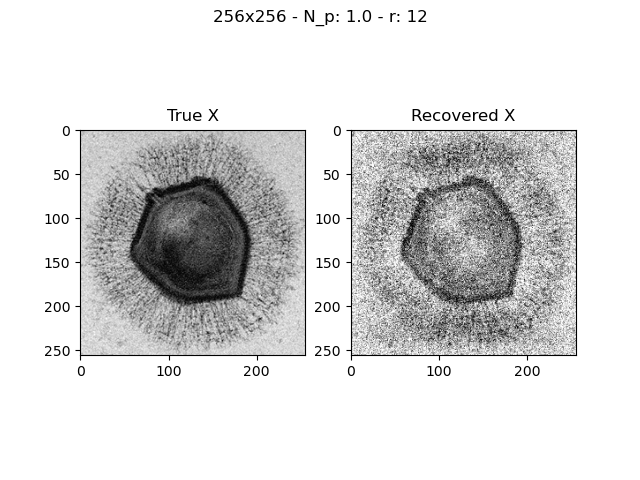
\includegraphics[width=0.45\textwidth]{img/fft/recover-256-1.png}
  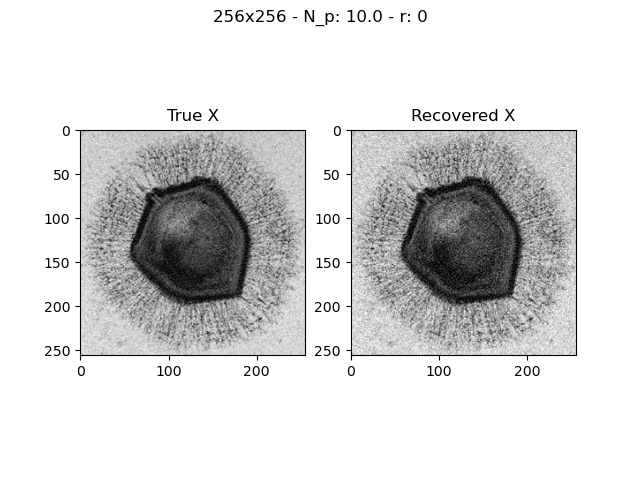
\includegraphics[width=0.45\textwidth]{img/fft/recover-256-10.png}
\end{center}
\vspace*{-12pt}
\begin{itemize}
\item MLE: $X^* = \textrm{arg max}_{X} \ p(X | \tilde{Y}, N, R,
  r)$
\item Bayesian estimate: $\widehat{X} = \mathbb{E}[X \mid \tilde{Y},
  N, R, r]$
\end{itemize}

  
% \sld{Time Series Autoregressive: AR(1)}
% % 
% \begin{stancode}
%   data {
%     int<lower=0> N;
%     vector[N] y;
%   }
%   parameters {
%     real alpha;
%     real beta;
%     real<lower=0> sigma;
%   }
%   model {
%     y[2:N] ~ normal(alpha + beta * y[1:N-1], sigma);
%     alpha ~ normal(0, 1);  beta ~ normal(0, 1);
%     sigma ~ lognormal(0, 1);
%   }
% \end{stancode}


\sld{Availability \& Usage}
\begin{subitemize}
\item \textit{Platforms:} \ Linux, Mac OS X, Windows
  \vspace*{-4pt}
\item \textit{Interfaces:} \ R, Python, Julia, MATLAB, Shell, C++
  \vspace*{-4pt}
\item \textit{Developers (academia \& industry):} 40+ \ {\small (10+ FTEs)}
  \vspace*{-4pt}
\item \textit{Users:}\ hundreds of thousands
  \vspace*{-4pt}
\item \textit{Companies using:} \ hundreds or thousands
  \vspace*{-4pt}
\item \textit{Downloads:}\ millions
  \vspace*{-4pt}
\item \textit{User's Group:} \ 5000+ registered; 30 posts \& 20K views/day
  \vspace*{-4pt}
\item \textit{Books using:} \ 10+
  \vspace*{-4pt}
\item \textit{Courses using:} \ 100+ (5+ on YouTube)
  \vspace*{-4pt}
\item \textit{Case studies about:} 100+
  \vspace*{-4pt}
\item \textit{Articles using:} \ 20,000+ (500+ just on Covid!)
  \vspace*{-4pt}
\item \textit{Conferences:} 4 (800+ attendance)
\end{subitemize}

\sld{Some published applications}
% 
\begin{subitemize}
\item \myemph{Physical sciences}: {\footnotesize
    astrophysics, statistical mechanics, particle physics, (organic) chemistry, geology, oceanography, climatology, biogeochemistry, materials science, $\ldots$
  }
  \vspace*{-3pt}
\item \myemph{Biological sciences}: {\footnotesize
    molecular biology, clinical drug trials, entomology, pharmacology,
    toxicology, opthalmology, neurology, genomics, agriculture, botany, fisheries,
    epidemiology, population ecology, neurology, psychiatry, $\ldots$
  }
  \vspace*{-3pt}
\item \myemph{Social sciences}: {\footnotesize
    econometrics (macro and micro), population dynamics, cognitive
    science, psycholinguistics, social networks, political science,
    survey sampling, anthropology, sociology, social work, $\ldots$
  }
  \vspace*{-3pt}
\item \myemph{Other}: {\footnotesize education, public health, A/B testing,
    government, finance, machine learning, logistics, electrical engineering,  transportation, actuarial science, sports, advertising, marketing, $\ldots$}
\end{subitemize}

\sld{Industries using Stan}
\vspace*{3pt}
\begin{subitemize}
\item \myemph{marketing attribution}: Google, Domino's Pizza, Legendary Ent.
\item \myemph{demand forecasting}: Facebook, Salesforce
\item \myemph{financial modeling}: Two Sigma, Point72
\item \myemph{pharmacology \& CTs}: Novartis, Pfizer, Astra Zeneca
\item \myemph{(e-)sports analytics}: Tampa Bay Rays, NBA, Sony Playstation
\item \myemph{survey sampling}: YouGov, Catalist
\item \myemph{agronomy}: Climate Corp., CiBO Analytics
\item \myemph{real estate pricing models}: Reaktor
\item \myemph{industrial process control}: Fero Labs
\end{subitemize}


\sld{Why is Stan so Popular?}
\vspace*{3pt}
\begin{subitemize}
\item \myemph{Community}: large, friendly, helpful, and sharing
\item \myemph{Documentation}:  novice to expert; breadth of fields
\item \myemph{Robustness}:  industrial-strength code; user diagnostics
\item \myemph{Flexibility}:  highly expressive language;  large math lib
\item \myemph{Portability}: popular OS, language, and cloud support
\item \myemph{Extensibility}: developer friendly; derived packages
\item \myemph{Speed}:  $2-\infty$ orders of magnitude faster
\item \myemph{Scalability}:  orders of magnitude more scalable than previous
\item \myemph{Openness}: permissive code and doc licensing
\end{subitemize}

\sld{Start with a Real Motivation}

\begin{itemize}
\item a reason for people to use your project (speed, scalability,
  ease of use, portability, robustness, functionality, etc.)
\item if you alleviate a pain point, your tool will be used
\item $\ldots$\ as long as it doesn't cause more collateral pain
\item January 2010: Andrew Gelman can't fit the models in his and
  Jennifer Hill's hierarchical regression book
  in BUGS or express them in lme4
\item so he hires two computer scientists with industrial coding
  experience (me \& Matt Hoffman) to try to figure it out
\item we failed to do that for several reasons $\ldots$
\end{itemize}

\sld{Faster Horses}

\begin{itemize}
\item There's an apocryphal story that Henry Ford once said that
  if he'd asked his customers what they wanted, they'd have said
  \myemph{faster horses}.
\item the point is \myemph{not to ignore your customers}
\item it's to \myemph{figure out what they really want} (faster, easier travel)
\item After souping up JAGS (C++ version of BUGS), Matt realized
  better engineering on JAGS was like breeding faster horses
\item After studying lme4, I realized we needed a more expressive
  language than a generalized lme4
\end{itemize}

\sld{Step 1: Ask the Community}
\begin{itemize}
\item Andrew has a ridiculously popular blog, {\slshape Statistical
    Statistical Modeling, Causal Inference, and Social Science}
\item So I asked for help in terms of where to look for more scalable
  samplers
\item Word on the street was Hamiltonian Monte Carlo
\item but it's almost impossible to tune
\item and it requires gradients
\end{itemize}
  

\sld{Pain Point 2: Tuning HMC}
\begin{itemize}
\item HMC is really really hard to tune
\item this time, nobody had any good ideas
\item Andrew formulated the goal as maximizing expected square jump
  distance and tuning acceptance
\item Matt started thinking about the U-turn idea to avoid waste
\item then he worked out how to maintain detailed balance
\item and add bias to get draws close to half an orbit
\item this was all before we had any users
\end{itemize}


\sld{NUTS vs.\ Gibbs and Metropolis samplers}
\vspace*{-6pt}
\begin{center}
  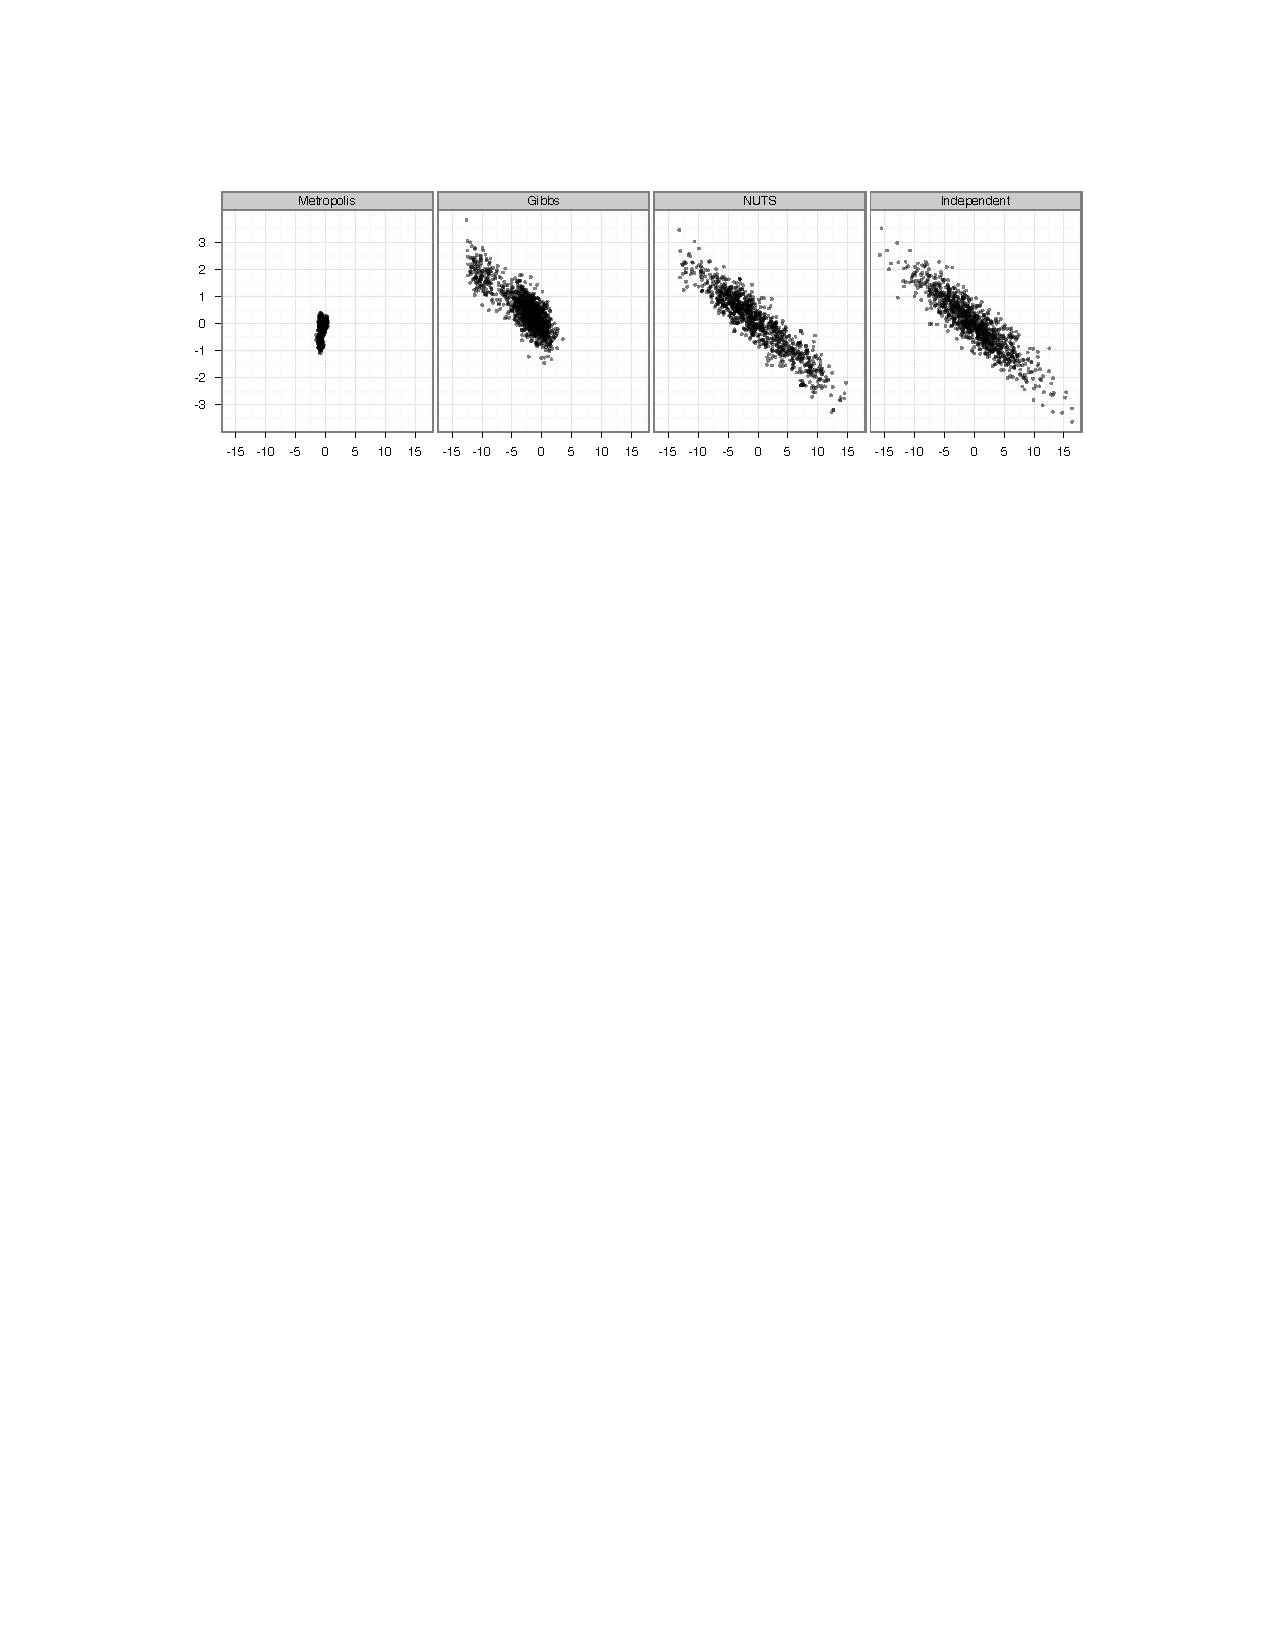
\includegraphics[width=0.8\textwidth]{img/nuts-vs.pdf}
\end{center}
\vspace*{-10pt}
\begin{subitemize}
\item \small Two dimensions of highly correlated 250-dim normal
\item \small \myemph{1,000,000 draws} from Metropolis and Gibbs (thin to 1000)
\item \small \myemph{1000 draws} from NUTS; 1000 independent draws
  \item HMC is $\mathcal{O}(N^{5/4})$ in dimension
    vs.\ Gibbs/Metropolis $\mathcal{O}(N^2)$
\end{subitemize}


\sld{Pain Point 3: Derivatives}
\begin{itemize}
\item I blegged again for help in computing gradients
\item Word on the street was automatic differentiation
  \begin{subitemize}
  \item we thought they meant finite differences
  \item but did a Wikipedia search and learned it was generalized
    backpropagation
  \end{subitemize}
\end{itemize}

\sld{Autodiff engineering}
\begin{itemize}
  \item this was before TensorFlow, PyTorch, or JAX
\item existing tools in 2011 were not well engineered
\item for either dynamic gradient performance or extension
\item Matt and I put our industry background to use and engineered a
  better C++ version 
\item using a modern lazy adjoint-Jacobian design
\item I named the first repo \texttt{agrad} 
\end{itemize}

\sld{Horses for courses}
\begin{itemize}
\item after TensorFlow and PyTorch hit the scene, we started planning
  for being overtaken
\item $\ldots$ \ but it still hasn't happened
\item big neural networks can exploit SIMD instructions, typical
  statistical models cannot
\item that gives us very different optimization goals
\item they're much faster on GPU and we're much faster on CPU (as
  reported by Google's TensorFlow team)
\item still improving (most recently, matrix memory locality)
\end{itemize}

\sld{Identify a point of entry}
\begin{itemize}
\item You need to solve at least one problem well
\item For us, it was hierarchical generalized linear models.
\item Just better solvers for those would be a big win
\item Work very hard and focus on an early win
  \begin{subitemize}
    \item for Stan, it was a PK/PD non-linear mixed effects model for
      a Phase I clinical trial with Novartis
    \end{subitemize}
  \item Daniel and I spent 6 months optimizing C++ (template
    traits, vectorizing, expression templates, checkpointing, analytic
    gradient unfolding) until Stan was faster than JAGS on its own example
    models (all small scale) 
\end{itemize}

\sld{It can be incremental}
\begin{itemize}
\item Most projects are not very innovative
\item Our autodiff is a better engineered version of Trilinos Sacado
\item Our language is a generalized, typed version of BUGS
\item Our sampler is an adaptive form of HMC (OK, that's innovative)
\end{itemize}

\sld{Your grain of salt}
\begin{itemize}
\item We did a lot of this consciously, but this report is pure hindsight
\item If you haven't taken your grain of salt yet, please do
  \vspace*{12pt}
\item It's hard to admit, but ventures like this require \myemph{a lot of
    luck}, especially \myemph{good timing}
\end{itemize}

\sld{Marketing and sales}
\begin{itemize}
\item Your project won't sell itself any more than your paper will
\item We have Andrew Gelman's bully pulpit---the blog
  \begin{subitemize}
    \item daily blog posts get 10K+ views including top statisticians
    \item Andrew also wrote the standard textbook and updated it to Stan
    \end{subitemize}
\item When Gelman puts you in his textbooks and blogs about you
  non-stop, people in the Bayes comp stats world listen
\item We also did lots of meetups, lectures, hackathons, etc. to get
  the word out
\end{itemize}

\sld{Why hadn't it been done before?}
\begin{itemize}
\item HMC is hard to tune
\item Hand-derived gradients are too big an ask
\item Autodiff at the time was primitive
\item Language and compiler design is hard
\item Constrained parameters are painful for HMC
  \begin{subitemize}
  \item Stan automates changes of variables
  \item gradients of log absoute Jacobian determinants
  \item working with Meenal Jhajaria (CCM intern) this summer
    comparing transform statistical \& computational efficiency
  \end{subitemize}
\end{itemize}

\sld{Assemble the right team}
\begin{itemize}
\item Previous efforts used statisticians exploring limited
  applications and with no CS experience
  \begin{subitemize}
  \item epidemiologists built BUGS and JAGS
  \item the BUGS devs said on record that if they
    could code C++, they'd have gone into finance
  \item R was a terrible role model as language \& community
  \end{subitemize}
\item Our project started day one with two \myemph{crack statisticians}
  (Gelman and Ben Goodrich),
\item plus three \myemph{industrially trained computer scientists} (me and Matt
  plus Daniel Lee)
\item and two years of financial runway in the form of grants
\end{itemize}

\sld{Reassemble the team}
\begin{itemize}
\item Grad students and postdocs come and go
\item So do software engineers once trained (industry pays better)
\item Need to keep recruiting devs to ensure project continuity
\item Pair programming is great for bringing up to speed
\item Tutorial onboarding docs are also critical
\item As is being welcoming and prioritizing new contributions
\end{itemize}

\sld{Support individual users}
\begin{itemize}
\item \myemph{Documentation} is necessary, but \myemph{not sufficient}
\item Need to \myemph{help individuals} on message boards, at meetups, $\ldots$
  \begin{subitemize}
  \item make sure user queries messages get answered in a timely
    fashion
  \item if they can't install your software or figure out how to use
    it, they will go away
  \end{subitemize}
\item Helping on message boards is rewarding (also learn a lot)
\item But it's very draining until it \myemph{bootstraps to self-sustaining}
  (thousands of visitors)
\end{itemize}

\sld{Go with an open license}
\begin{itemize}
\item This used to be more contentious
\item MIT- and BSD-like licenses seem to have won over copyleft
  licenses like GPL
\item Everyone asks why we give it away free to industry
  \begin{subitemize}
  \item they give back in cash and in kind
  \item and your devs may wind up there soon and still want to use the
    system they built
  \item cool open source spinoffs like Prophet
  \end{subitemize}
\end{itemize}

\sld{Code Review}
\begin{itemize}
\item A tech manager friend of mine asked how we did code review.
\item I admitted we didn't.
\item Adding that was the single biggest quality boost we made
\item Two eyes are way better than one at spotting flaws
\item With review, at least two people understand each piece of code
\item It also keeps you honest knowing there will be a review
\end{itemize}


% \sld{Start with a vision, not a committee}
% \begin{itemize}
% \item good design comes out of coherent vision
% \item committees slow things down and drag things to the middle of the
%   road
% \end{itemize}

\sld{Earn trust through openness}
\begin{itemize}
\item Transparency and open discussion leads to trust (GitHub, forums,
  blog posts, etc.)
\item Find a way to be responsive
\item Underpromise and overdeliver
\item Admit errors, advertise and take responsibility (and patch!)
  bugs ASAP
\item Similar projects are your allies, not your enemies
\item If people understand your problems, they'll cut you slack
  \begin{subitemize}
  \item but things can be hard to explain to non-specialists (stats or CS)
  \end{subitemize}
\end{itemize}

\sld{Be very careful with comparisons}
\begin{itemize}
  \item If your project has advantages, you won't need detailed
    comparisons
  \item Comparing adaptive stochastic systems is a \myemph{Very Hard
      Thing}
  \item Be gracious to your competitors and they'll be gracious to you 
\end{itemize}
  
\sld{Your project depends on evangelists}
\begin{itemize}
\item You need to help the early adopters and they'll help others
\item Early adopters often become evangelists or devs
\item Don't be surprised when the evangelists oversell your project
\item User tutorials at conferences are good venues
\item Longer hands-on tutorials and multi-session classes are even better
\end{itemize}

\sld{Grow your process with your project}
\begin{itemize}
\item Move from Daniel and me back to back in an office
\item to dozens of devs communicating through forum posts, Slack,
  GitHub and small Zoom or in-person meetings
\item Need to keep continuous integration testing up to date
\item We grew into all this organically as the project grew.
\item We now have fancy things like syntax highlighting in markdown
  and Git and are even a language reported by GitHub
\end{itemize}

\sld{Support others building on your tooling}
\begin{itemize}
\item Hundreds of other packages built on Stan in R and Python
\item Derived projects are used more than Stan itself
\item It'll make your software better and expand your user base
\item Support other groups trying to build a better mousetrap
  \begin{subitemize}
  \item learn from them, or plan your project's retirement
  \item either way, it's good
  \end{subitemize}
\end{itemize}

\sld{High-level interfaces}
\begin{itemize}
\item To my surprise, some people find Stan challenging
\item For them, we have high-level interfaces
\item Most interfaces encapsulate whole models and data ingestion formats
  \begin{subitemize}
  \item Facebook built Prophet, a demand forecasting system
  \item Metrum built Torsten, a pharmacology modeling system
  \item others have distributed models (like Google's ad attribution)
  \end{subitemize}
\item Others encapsulate whole classes of models (rstanarm) or
  introduce sublanguages (brms)
\end{itemize}

\sld{Governance}
\begin{itemize}
\item Politics (group decision making) is hard
\item Want zone before techie zeal and academic reticence
\item I resisted being made benevolent dictator for life
\item But wrongly instituted module decision makers and a tech
  director
\item No siree, Bob. You really want to follow Apache and go with voting
\item which pushes politics to who votes on what
\end{itemize}

\sld{Scaling Out}
\begin{itemize}
\item Scaling up (at one institution) only goes so far
\item Embrace scaling out
\item We have ``centers'' in Helsinki, Ljubljana, and now two in NYC
  with Flatiron and Columbia
\item Support fully remote workers (we got used to online meets before Covid)
\end{itemize}

\sld{Measuring community is hard}
\begin{itemize}
\item Too many distribution channels
\item Too many bots and multiple downloads
\item What's a user?
  \begin{subitemize}
  \item current or one-time use?  classroom use?
  \item do you have to write the code or just run it?
  \item what about embedded uses?
  \end{subitemize}
\item Proxies include citations, books, classes, videos, stars on GitHub,
  contributing devs, user group clicks, etc. 
\item or mentions in the mainstream media
\end{itemize}

\sld{Naming}
\begin{itemize}
\item I named the initial repo \texttt{agrad}
\item Andrew really settled on Stan (for Stanislaw Ulam [and the Eminem song])
\item Hadley Wickham and I tried to convince him we wanted
  \begin{subitemize}
  \item zero hits on Google
  \item not spell corrected
  \end{subitemize}
\item The name ``Stan'' is unsearchable
\item but it's growing on me
\end{itemize}

\sld{Questions?}
\begin{itemize}
  \item To learn more, see: \texttt{https://mc-stan.org}
  \end{itemize}
  
\sld{Music and Cocktails?}
\begin{subitemize}
\item I hear Alex has assembled a band
\item and Jonathan is making Stanleys on the roof
\end{subitemize}
\begin{center}
  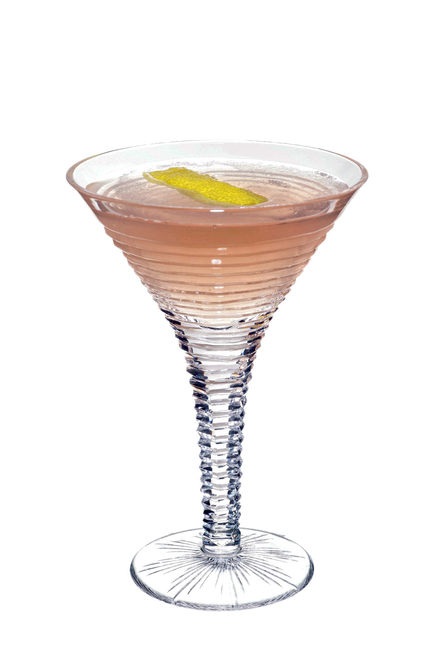
\includegraphics[width=0.3\textwidth]{img/stanley.jpeg}
\end{center}

\end{document}

